% Modelo de slides para projetos de disciplinas do Abel
\documentclass[10pt]{beamer}

\usetheme[progressbar=frametitle]{metropolis}
\usepackage{appendixnumberbeamer}
\usepackage[numbers,sort&compress]{natbib}
\bibliographystyle{plainnat}
\usepackage{booktabs}
\usepackage[scale=2]{ccicons}
\usepackage{xspace}
\newcommand{\themename}{\textbf{\textsc{metropolis}}\xspace}
%%%%%%%%%%%%%%%%%%%%%%%%%%%%%%%%%%%%%%%%%%%%
\usepackage[spanish,es-noshorthands]{babel}
% Paquete pdfpages incluye páginas completas de ficheros pdfs
\usepackage{pdfpages}
%TikZ 
\usepackage{pgf,tikz}
\usetikzlibrary{shapes,arrows}
% PGFPlots
\usepackage{pgfplots}
\pgfplotsset{width=6cm,compat=1.12} %{compat=yourversion}
%paquete chemfig: gráficos de química
\usepackage{chemfig}
%paquete Wrapfig
\usepackage{wrapfig}

%%%%%%%%%%%%%%%%%%%%%%%%%%%%%%%
\title{Inserción/edición y creación \\ de 
gráficos con \LaTeX{}}
% \subtitle{Subtítulo}
% \date{\today}
\date{}
\author{Óscar Sánchez Romero}
\institute{Dpto. Matemática Aplicada, UGR}
% \titlegraphic{\hfill\includegraphics[height=1.5cm]{logo.pdf}}
%%%%%%%%%%%%%%%%%%%%%%%%%%%%%%%%%%%
\begin{document}

\maketitle

\begin{frame}{Contenidos}
  \setbeamertemplate{section in toc}[sections numbered]
  \tableofcontents[hideallsubsections]
\end{frame}

\section{Introducción}

\subsection{Uso frecuente}
\begin{frame}[fragile]{Uso básico}
Todos sabemos que en un documento generado con \LaTeX{} podemos incorporar  gráficos  
\begin{figure}[h]
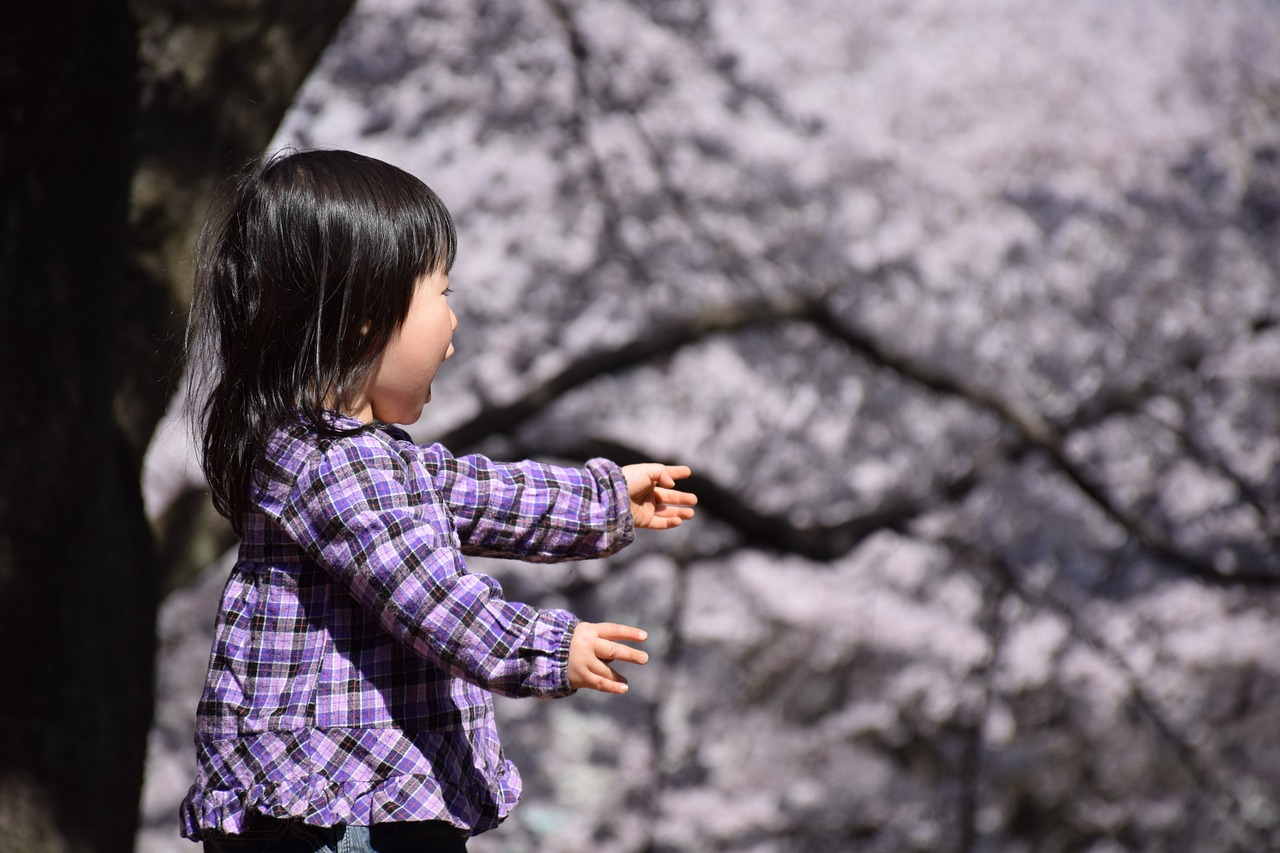
\includegraphics[width=0.3\textwidth]{../graficos/sorpresa.jpg} 
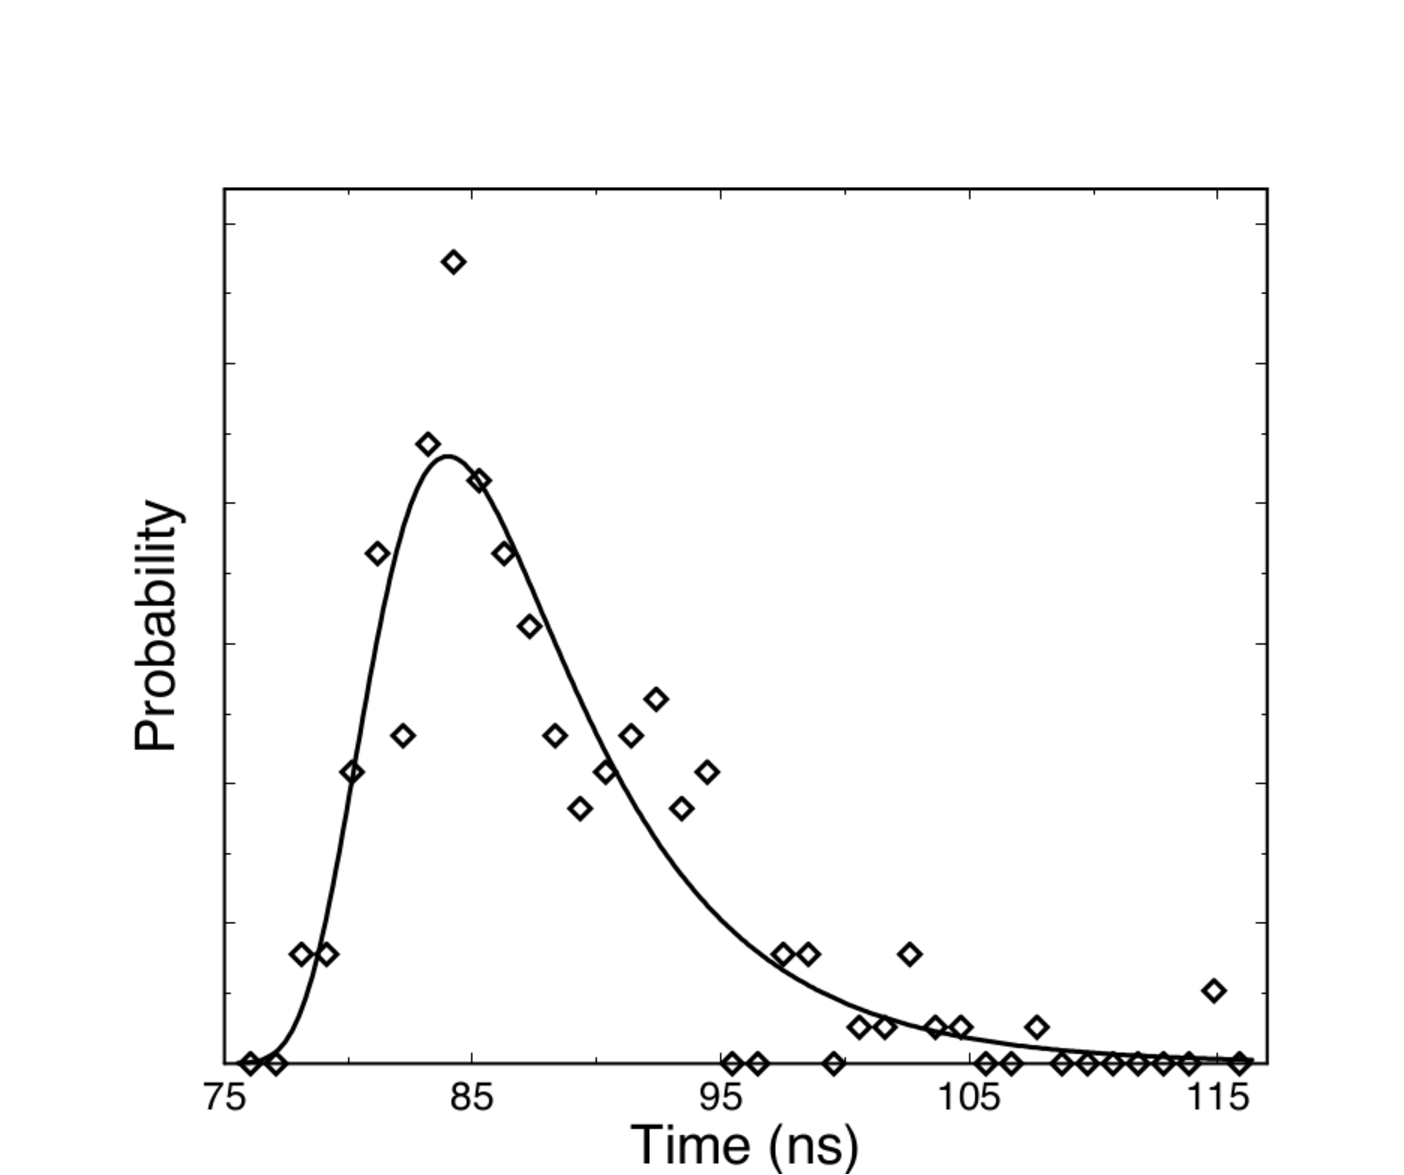
\includegraphics[width=0.3\textwidth]{../graficos/fig_9Vis.pdf}
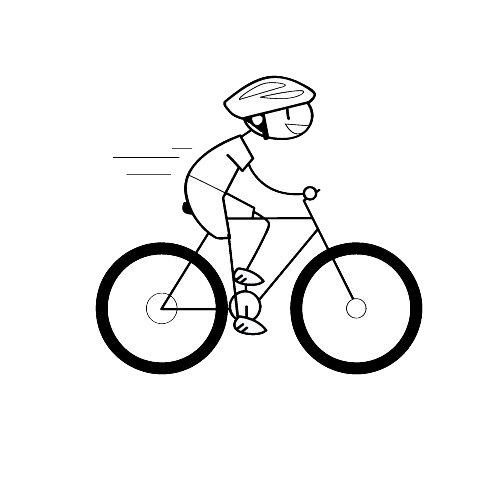
\includegraphics[width=0.3\textwidth]{../graficos/ciclista.png}
\caption{Caption general}
\label{figGeneral}
\end{figure}
\end{frame}
%%%%%%%%%%%%%%%%%%%%%%%%%%%%%%%%%%%%%%%%%%%%
\subsection{Uso no tan frecuente}
\begin{frame}[fragile]{Uso no tan frecuente}
Lo que no es tan conocido es que, al incorporarlos, permite editarlos ligeramente.
%\vspace{-1cm}
%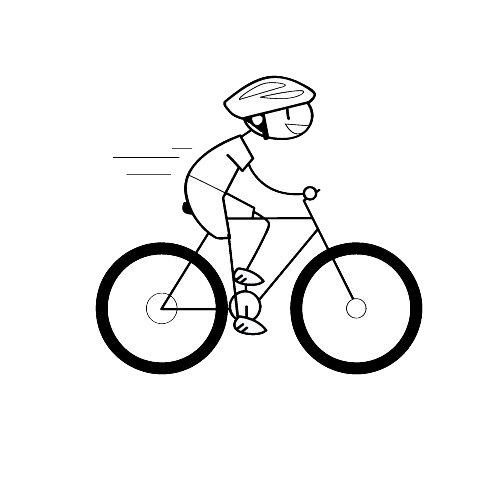
\includegraphics[angle=0, width=3cm]{./../graficos/ciclista}
\begin{figure}
\centering
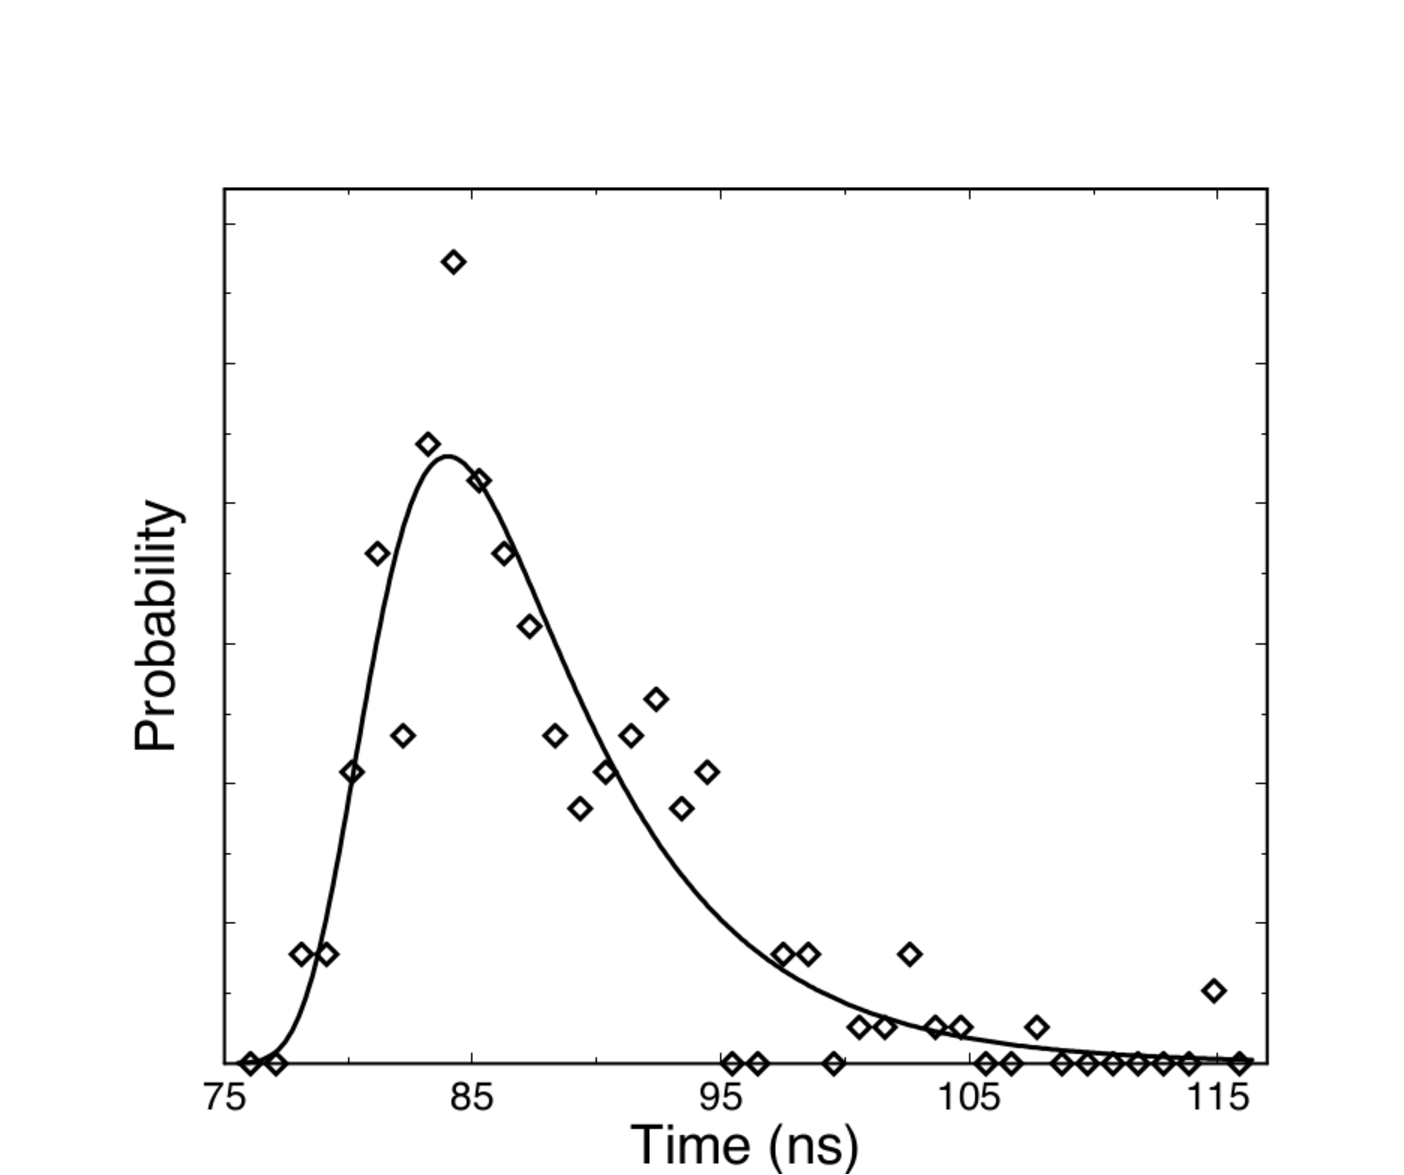
\includegraphics[width=6cm]{./../graficos/fig_9Vis}
\put(-90,5){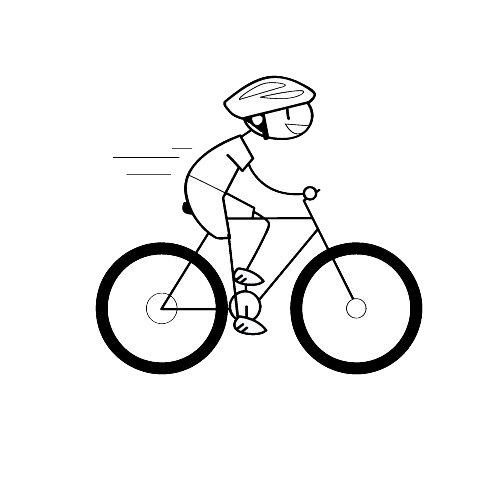
\includegraphics[angle=-10,scale=0.4]{./../graficos/ciclista}}
\caption{Redimensionar, girar y superponer imágenes}
\end{figure}
{\scriptsize OJO!  Requiere 
\href{https://docs.gimp.org/2.10/es/gimp-using-web-transparency.html}{\color{blue}fondo transparente} en la figura a superponer (objeto).}
\end{frame}
%%%%%%%%%%%%%%%%%%%%%%%%%%%%%%%%%%%%%%%%%%%%%%

\begin{frame}[fragile]{Uso no tan frecuente}
Lo que no es tan conocido es que, al incorporarlos, permite editarlos ligeramente.

\begin{figure}
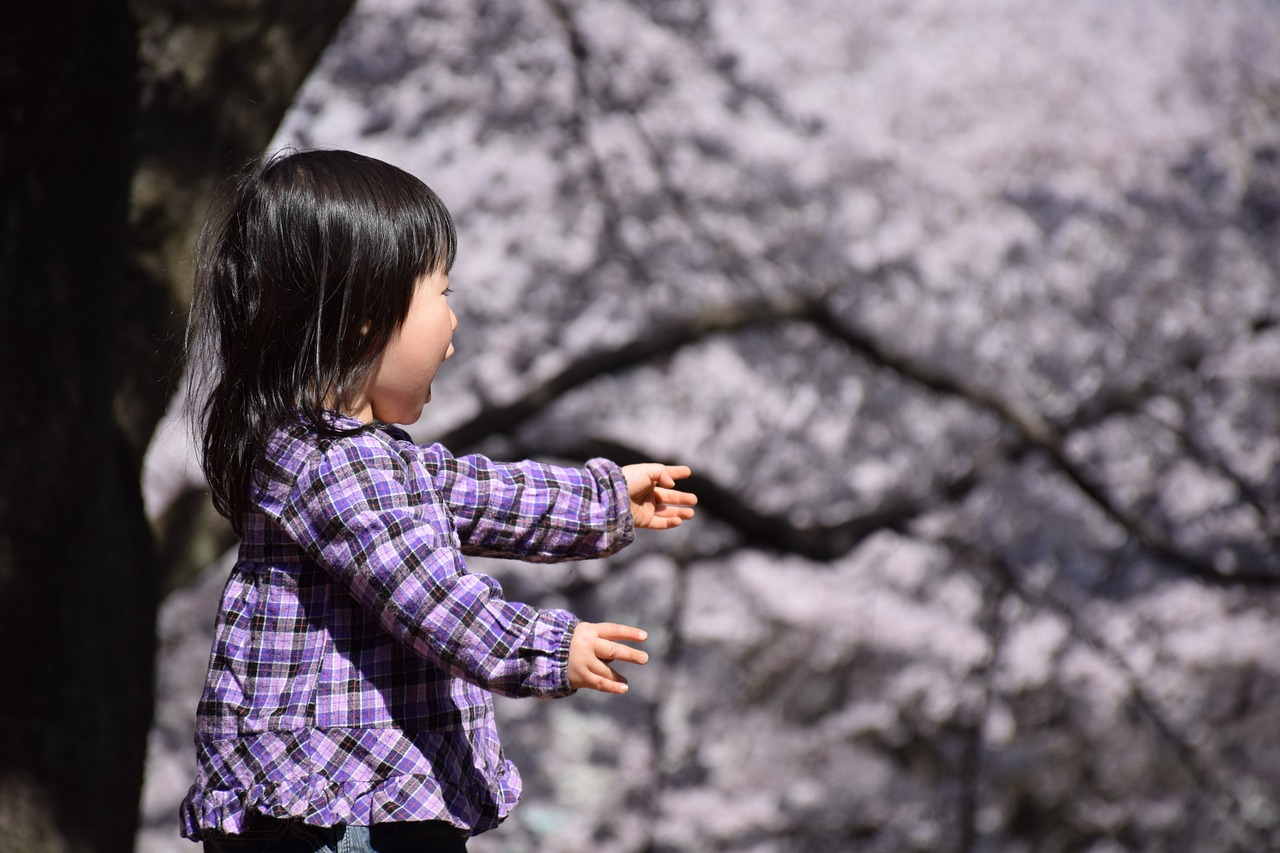
\includegraphics[trim = 50mm 0mm 190mm 40mm, clip,width=4.5cm]{./../graficos/sorpresa}
\hspace{-0.3cm}
\reflectbox{
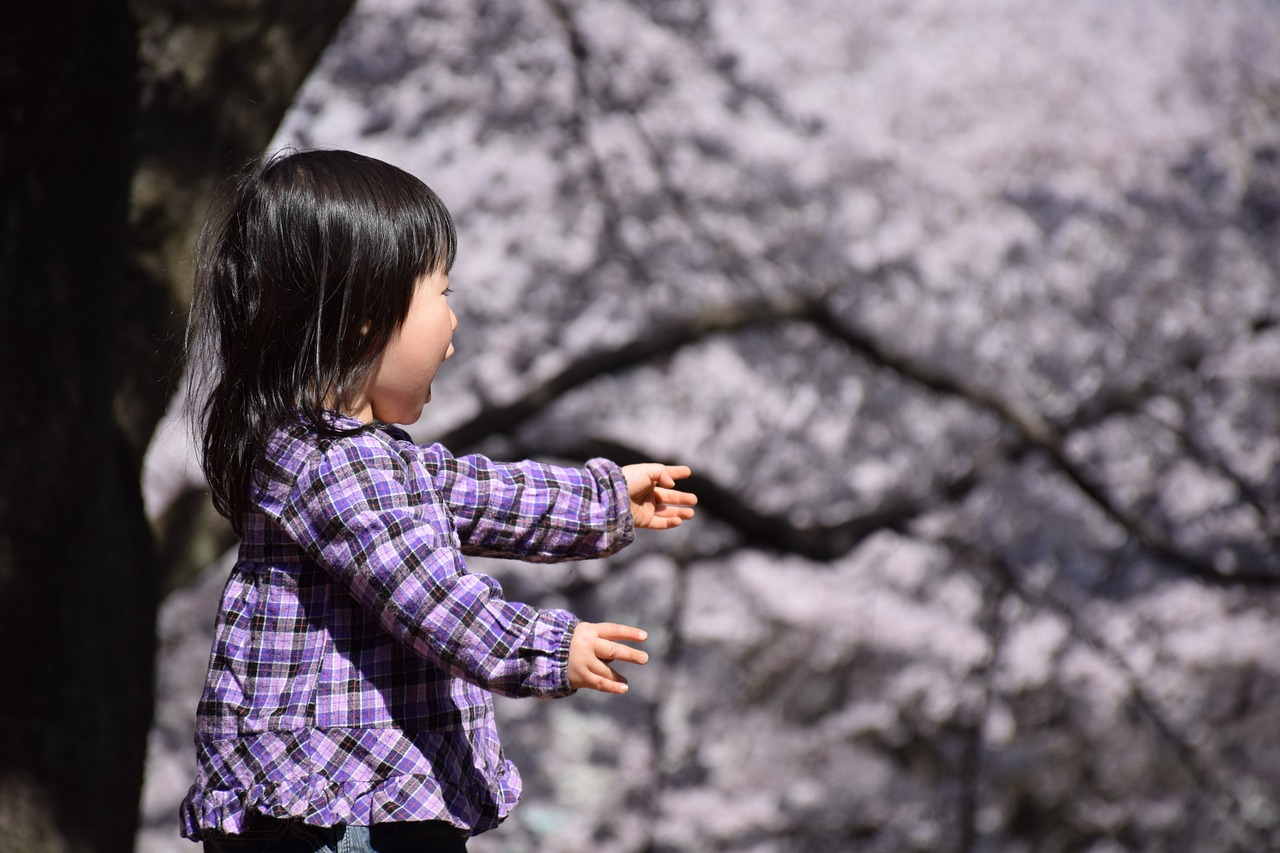
\includegraphics[trim = 50mm 0mm 190mm 40mm, clip,width=4.5cm]{./../graficos/sorpresa}
}
\put(-195,135){{\color{green}   \LARGE \textbf{Powered by \LaTeX}}}
\caption{Selección, simetrizar, incluir texto}
\end{figure}

\end{frame}


%%%%%%%%%%%%%%%%%%%%%%%%%%%%%%%%%%%%%%%%%%%%%
\begin{frame}{Gr\'aficos insertados vs generados}
%Cada vez recurrimos m\'as a representaciones gr\'aficas para ejemplificar. 

La inclusi\'on de muchos documentos gr\'aficos en un mismo documento \LaTeX $ $ tienen varios inconvenientes:
\begin{itemize}
\item Dan como resultado documentos muy pesados.
\item Pese a ello, la calidad de los gr\'aficos insertados no siempre es 
 \'optima.
 \end{itemize}

La soluci\'on que \LaTeX \ adopt\'o   hace tiempo es algo que est\'a hoy d\'ia muy de moda:
\begin{center}
Do it yourself (DIY)
\end{center}
%Esto es,  el propio \LaTeX \  interpreta una serie de instrucciones y genera el 
%gr\'afico.  Otra cosa distinta es c\'omo generamos dicho c\'odigo...
\begin{itemize}
\item {\small \color{red} Ventajas: }Alta calidad y ficheros con peso reducido.\\
\item {\small \color{red} Inconveniente:} inversión de tiempo de aprendizaje.
\end{itemize}
%por ejemplo este documento con $31$ gr\'aficas ocupa 438 KB!!!. }
\end{frame}



%%%%%%%%%%%%%%%%%%%%%%%%%%%%
\section{Inserción/edición de gráficos}
%%%%%%%%%%%%%%%%%%%%%%%%%%%%
\subsection{Preparación del gráfico}
\begin{frame}{Generalidades sobre formatos gr\'aficos}
\begin{block}{Mapas de bits} 
\begin{center}
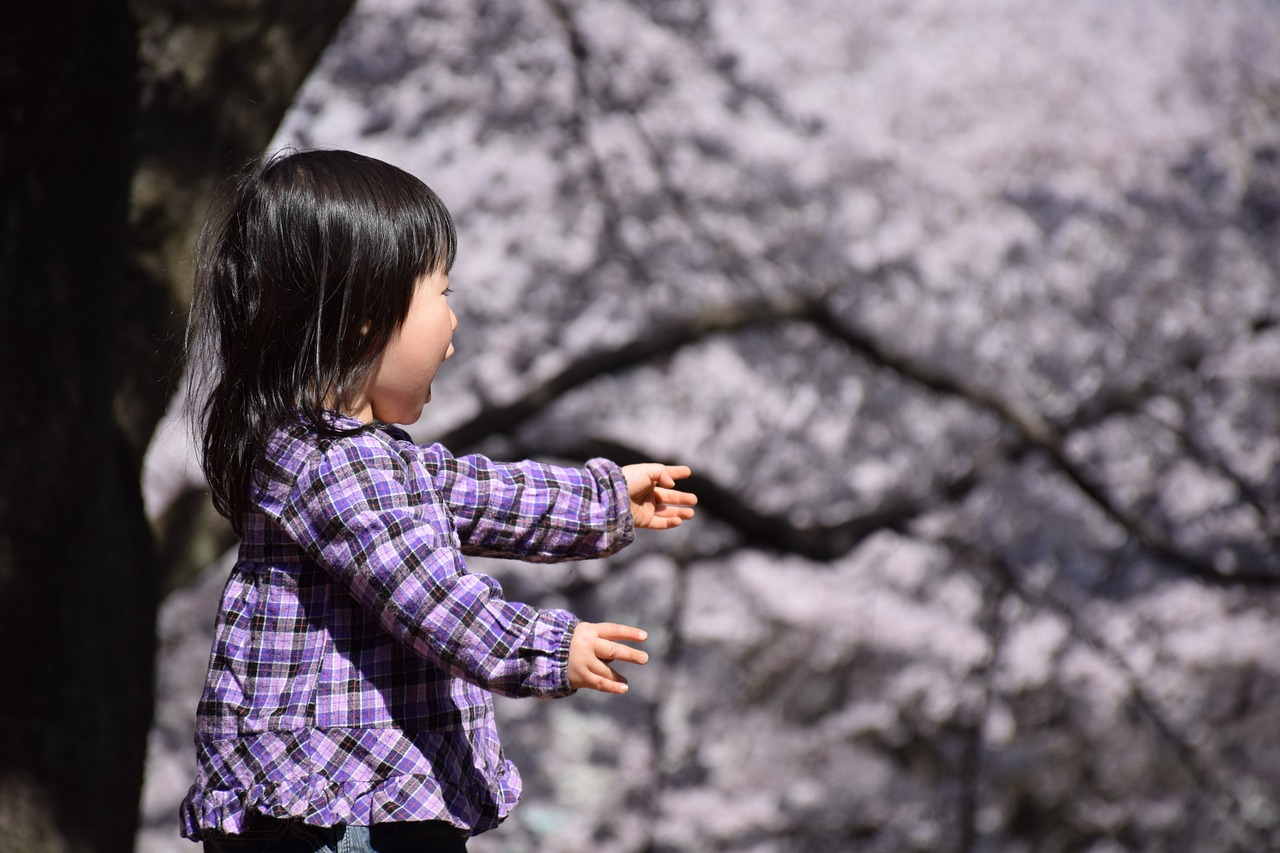
\includegraphics[width=7cm]{../graficos/sorpresa.jpg}
\end{center}
Extensiones: BMP, JPEG, GIF, PNG y TIFF. \\
{\small Desventaja: deformaciones al reescalar y gran tama\~no.}
\end{block}
\end{frame}
%%%%%%%%%%%%%%%%%%%%%%%%%%%%
\begin{frame}{Generalidades sobre formatos gr\'aficos}
\begin{block} {Gr\'aficos vectoriales} 
%\vspace{-1cm}
\begin{center}
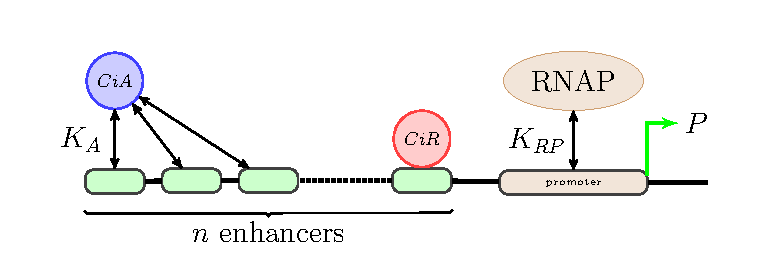
\includegraphics[width=10cm]{../graficos/bp2.pdf}
\end{center}
Extensiones: EPS, PDF, SVG, WMF \\
{\small Nota: !`Estos archivos pueden insertar mapas de bits! }
\end{block}
\end{frame}
%%%%%%%%%%%%%%%

\begin{frame}{Preparaci\'on de gr\'aficos para insertar en \LaTeX}
El formato del gr\'afico a insertar depende del compilador empleado:
\begin{enumerate}
\item \it{latex + dvips}  se requiere PS / EPS {\scriptsize(con \href{http://tex.stackexchange.com/questions/133786/no-boundingbox-error-message}{\color{blue}BoundingBox})}
\item \it {pdflatex} se requiere PNG {\scriptsize(mapas de bits simples)}, JPEG {\scriptsize(fotograf\'ias)} o PDF {\scriptsize(gr\'aficos vectoriales)}
\end{enumerate}

\vspace{0.5cm}
Esto requiere de programas espec\'ificos de transformaci\'on:
\begin{itemize}
\item {\sc EPS a PDF}: \href{http://tug.org/epstopdf/}{\color{blue}epstopdf}
%\item {\sc JPEG a EPS}: \href{http://www.pdflib.com/download/free-software/jpeg2ps/}{jpeg2ps}
\item {\sc Todo a Todo}: \href{http://www.inkscape.org/es/}{\color{blue}Inkscape}, 
\href{http://www.imagemagick.org}{\color{blue}ImageMagick} o \href{http://www.gimp.org/}{\color{blue}Gimp}
\item ........
\end{itemize}
Ver detalles en \cite{ManualLatexWikilibros}.
\end{frame}

%%%%%%%%%%%%%%%%%%%%%%%%%%%%%%%%%%%%%%%%%%
\subsection{Inserci\'on de un gr\'afico}
%%%%%%%%%%%%%%%%%%%%%
\begin{frame}[fragile]{Insertar el gr\'afico como una figura}
Declaraci\'on del paquete graphicx en el pre\'ambulo:
\begin{verbatim}\usepackage{graphicx} \end{verbatim}

Inserci\'on del gr\'afico en el documento:
\begin{verbatim}
\begin{figure}
  \centering
  \includegraphics[parametros]{nombregrafico}
  \caption{Leyenda bajo el grafico}
  \label{fig:etiqueta}
\end{figure}
\end{verbatim}
Mediante los par\'ametros se puede modificar el aspecto, lo que 
nos permite editarlos ligeramente.
\end{frame}

%%%%%%%%%%%%%%%%%%%%%%%%%%%%%%%%%%%%%%%%%%
\subsection{Edici\'on de un gr\'afico}
\begin{frame}[fragile]{Parámetros para modificar una figura}
Parámetros empleados más usualmente:
\begin{itemize}
    \item \verb|scale=0.5 | \hfill escala el tamaño a la mitad
    \item \verb|height=5cm | \hfill fija la anchura del gráfico a 5cm
    \item \verb|width=0.5\textwidth | \hfill anchura = mitad del espacio para texto.
    \item \verb|angle=90 |\hfill  gira la imagen 90 grados.
    \item \verb|trim = 10mm 5mm 50mm 55mm, clip| \hfill Recorta la imagen quitando
\verb|trim = <left> <lower> <right> <upper> | \hfill 10mm por izda,...
    \item \verb|draft| \hfill no se incluye el gráfico pero deja el espacio apropiado.
\end{itemize}
\vspace{1cm}
Para profundizar ver documentaci\'on paquete graphicx \cite{DocGraphicx} .
\end{frame}
%%%%%%%%%%%%%%%%%%%%%%%%%%%%%%%%%%%%%%%%%%
\begin{frame}[fragile]{Localización de la figura en el texto}
El entorno figure es flotante, esto es, \LaTeX{} ``decide''
dónde lo pone. Si queremos controlar este proceso tenemos varias 
opciones:
\begin{itemize}
    \item Control débil del entorno \verb|figure| con parámetros 
    de control h, b, t. 
    \item Empleo del entorno \verb|wrapfigure| \cite{wrapfigure} gracias al paquete \verb|wrapfig|.
    \item Empleo del parámetro H del paquete \verb|float|.
    \item Usar \verb|includegraphics| sin entorno \verb|figure|. \hfill (No recomendable)
\end{itemize}
\vspace{1cm}
Ver detalles en \href{https://www.overleaf.com/learn/latex/Positioning_images_and_tables}{\color{blue}ayuda de OverLeaf}.
\end{frame}


%%%%%%%%%%%%%%%%%%%%%%%%%%%%
\begin{frame}[fragile]{Otra utilidad: inclusión páginas completas pdf}
\vspace{-4cm}
\begin{wrapfigure}{r}{6cm}
\hspace{0.5cm}

\includegraphics[width=5.cm]{../graficos/DeclaraciondeOriginalidadTFG.pdf}
\end{wrapfigure}
\vspace{1cm}
El paquete pdfpages \cite{pdfpages} permite incluir páginas seleccionadas de un pdf en un documento \LaTeX{}. 

{\scriptsize Utilidad: generar documentación acreditativa, \\incluir declaraciones en documentos, etc...}

\begin{verbatim}
\includepdf[]{file.pdf}
\end{verbatim}
\end{frame}




%%%%%%%%%%%%%%%%%%%%%%%%%%%%%%%%%%%%%%%%%%%%%%%
\section{Creación de gráficos con LaTeX}
%%%%%%%%%%%%%%%%%%%%%%%%%%%%%%%%%%%%%%%%%

%%%%%%%%%%%%%%%%%%%%%%%%%%%%%%%%%%%%%%%%%%
\begin{frame}[fragile]{Gr\'aficos con PSTricks y TikZ}
Tanto \href{http://www.ctan.org/pkg/pstricks}{\color{blue}PSTricks} como \href{http://www.texample.net/tikz/}{\color{blue}PGF-TikZ} son paquetes de LaTeX que permiten hacer casi cualquier cosa mediante un gran abanico de comandos espec\'ificos.

Podemos sacar provecho de ellos de v\'arias maneras:
\begin{enumerate}
\item Escribiendo nosotros directamente los c\'odigos (siempre que estemos dispuestos a invertir nuestro tiempo en ello). Hay disponibles numerosos manuales, y ejemplos:
\begin{itemize}
\item \href{http://www.texample.net/tikz/examples/}{\color{blue}http://www.texample.net/tikz/examples/}
\item \href{http://tug.org/PSTricks/main.cgi?file=examples}{\color{blue}http://tug.org/PSTricks/main.cgi?file=examples}
\end{itemize}
\item Empleando paquetes que facilitan su uso como PGFPlots.
\item Crear los gr\'aficos con otros programas y exportarlos a TikZ.
\end{enumerate}


\vspace{0.5cm}
{\small Observaci\'on:
Aunque PSTricks no es compatible con PDFLaTeX, existen versiones (spt-pdf o pdftricks)
que sí lo son.}
\end{frame}

%%%%%%%%%%%%%%%%%%%%%%%%%%%%%%%%%%%%%%%%%%
\begin{frame}[fragile]{Filosofía básica TikZ}
\begin{wrapfigure}{r}{4cm}
\begin{tikzpicture}[scale=1]
\draw[help lines] (0,0) grid (3,3);
\draw[->] (0,0) -- (2,2.5);
\end{tikzpicture}
\caption{Gr\'afico sencillo TikZ}
\end{wrapfigure}
$ $
\begin{verbatim}
\begin{tikzpicture}
\draw[help lines]  (0,0) grid (3,3);
\draw[->]  (0,0) -- (2,2.5);
\end{tikzpicture}
\end{verbatim}
\vspace{2cm}
\href{https://cremeronline.com/LaTeX/minimaltikz.pdf}{\color{blue}A very minimal introduction to TikZ}\\
\href{https://es.wikibooks.org/wiki/Manual_de_LaTeX/Inclusi%C3%B3n_de_gr%C3%A1ficos/Gr%C3%A1ficos_con_TikZ}{\color{blue}Manual de LaTeX/Inclusión de gráficos/Gráficos con TikZ}
\end{frame}
%%%%%%%%%%%%%%%%%%%%%%%%%%%%%%%%%%%%%%%%%%
\begin{frame}[fragile]{Filosofía básica TikZ}
\begin{wrapfigure}{r}{4cm}
\begin{tikzpicture}
\draw[<->, line width = 1pt]  (3.5,0) --(0,0) -- (0,1.5);
\draw [blue, domain=0:pi]  plot (\x, {sin(\x r)*exp(\x/exp(2*pi))});
\end{tikzpicture}
\caption{Gr\'afico sencillo TikZ}
\end{wrapfigure}
$ $
\vspace{1cm }
\begin{verbatim}
\begin{tikzpicture}
\draw[<->, line width = 1pt] 
(3.5,0) --(0,0) -- (0,1.5);
\draw [blue, domain=0:pi] 
plot (\x, {sin(\x r)*exp(\x/exp(2*pi))});
\end{tikzpicture}
\end{verbatim}
%\vspace{2cm}
%\href{https://cremeronline.com/LaTeX/minimaltikz.pdf}{\color{blue}A very minimal introduction to TikZ}\\
%\href{https://es.wikibooks.org/wiki/Manual_de_LaTeX/Inclusi%C3%B3n_de_gr%C3%A1ficos/Gr%C3%A1ficos_con_TikZ}{\color{blue}Manual de LaTeX/Inclusión de gráficos/Gráficos con TikZ}
\end{frame}

%%%%%%%%%%%%%%%%%%%%%%%%%%%%%%
\begin{frame}[fragile]{Funcionalidades específicas: árboles}

\begin{tikzpicture}[every node/.style={rectangle, fill=blue!20!white}]
\node {Animalia} [sibling distance=6cm]
child {node {Chordata}
	child {node {Vertebrata} [sibling distance=1.5cm]
		child {node {Mammalia}}
		child {node {Aves}}
		}
	}
child {node {Arthoropoda} [sibling distance=4cm]
	child {node {Mandibulata}[sibling distance=2cm]
		child {node {Insecta}}
		child {node {Crustacea}}
		}
	child {node {Chelicerata}
		child {node {Arachnida}}
		}
	};
\end{tikzpicture}
%
\end{frame}

%%%%%%%%%%%%%%%%%%%%%%%%%%%%%%
\begin{frame}[fragile]{Funcionalidades específicas: diagramas de flujo}

% Define block styles
\tikzstyle{decision} = [diamond, draw, fill=blue!20, 
    text width=3.5em, text badly centered, node distance=3cm, inner sep=0pt]
\tikzstyle{block} = [rectangle, draw, fill=blue!20, 
    text width=4em, text centered, rounded corners, minimum height=3em]
\tikzstyle{line} = [draw, -latex']
\tikzstyle{cloud} = [draw, ellipse,fill=red!20, node distance=3cm,
    minimum height=2em]
    
\begin{tikzpicture}[yscale=0.5,node distance = 2cm, auto]
    % Place nodes
    \node [block] (init) {\footnotesize initialize model};
    \node [cloud, left of=init] (expert) {\footnotesize expert};
    \node [cloud, right of=init] (system) {\footnotesize system};
    \node [block, below of=init] (identify) {\footnotesize identify candidate models};
    \node [block, below of=identify] (evaluate) {\footnotesize evaluate candidate models};
    \node [block, left of=evaluate, node distance=3cm] (update) {\footnotesize update model};
    \node [decision, below of=evaluate] (decide) {\footnotesize is best candidate better?};
    \node [block, right of=decide, node distance=3cm] (stop) {\footnotesize stop};
    % Draw edges
    \path [line] (init) -- (identify);
    \path [line] (identify) -- (evaluate);
    \path [line] (evaluate) -- (decide);
    \path [line] (decide) -| node [near start] {yes} (update);
    \path [line] (update) |- (identify);
    \path [line] (decide) -- node {no}(stop);
    \path [line,dashed] (expert) -- (init);
    \path [line,dashed] (system) -- (init);
    \path [line,dashed] (system) |- (evaluate);
\end{tikzpicture}

\end{frame}



%%%%%%%%%%%%%%%%%%%%%%%%%%%%%%
\subsection{Uso de paquetes específicos}
\begin{frame}[fragile]{Paquete pgfplots}
Un primer ejemplo puede ser \href{http://pgfplots.net}{\color{blue}pgfplots} para representar funciones y datos.
\begin{wrapfigure}{r}{5cm}
\begin{tikzpicture} \begin{axis}[
    title={$x \exp(-x^2-y^2)$},
    xlabel=$x$, ylabel=$y$,
    small,
] \addplot3[
    surf,
    domain=-2:2,
    domain y=-1.3:1.3,
]
    {exp(-x^2-y^2)*x};
\end{axis}
\end{tikzpicture}
\caption{Gr\'afico tridimensional}
\end{wrapfigure}
$ $ %\vspace{1cm}
\begin{verbatim}
\begin{tikzpicture} 
\begin{axis}[
    title={$x \exp(-x^2-y^2)$},
    xlabel=$x$, ylabel=$y$,
    small] 
\addplot3[surf,
    domain=-2:2,
    domain y=-1.3:1.3
]{exp(-x^2-y^2)*x};
\end{axis}
\end{tikzpicture}
\end{verbatim}
\end{frame}
%%%%%%%%%%%%%%%%%%%%%%%%%%%%%
\begin{frame}[fragile]{Uso de paquetes específicos}
Este uso se está extendiendo en \'areas distintas a la Física o las Matemática como por ejemplo el paquete chemfig \cite{Chemical} en \href{https://www.ctan.org/search/index?phrase=chemistry&offset=48&max=16}{\color{blue}Química}
\begin{wrapfigure}{r}{4cm}
\chemfig{-(-[1]O^{\ominus})=[7]O}

\chemfig{C(-[:0]H)(-[:90]H)(-[:180]H)(-[:270]H)}
\caption{Gr\'aficos química}
\end{wrapfigure}
\begin{verbatim}
\chemfig{-(-[1]O^{\ominus})=[7]O}
\end{verbatim}
\vspace{1cm}
\begin{verbatim}
\chemfig{C(-[:0]H)(-[:90]H)
(-[:180]H)(-[:270]H)}
\end{verbatim}
\end{frame}




%%%%%%%%%%%%%%%%%%%%%%%%%%%%%%
\begin{frame}[fragile]{Uso avanzado: sitios de interés}
Puesto que es imposible mostrar paquetes de interés para una 
audiencia heterogénea lo mejor es mostrar dónde y cómo localizarlos

\href{https://www.ctan.org}{\color{blue}https://www.ctan.org}

\href{https://es.wikibooks.org/wiki/Manual_de_LaTeX/Inclusión_de_gráficos/Gráficos_con_TikZ}{\color{blue}Wikibooks: Gráficos con Tikz}

\href{http://www.texample.net/tikz/examples/}{\color{blue}http://www.texample.net/tikz/examples/}

\href{https://tex.stackexchange.com/questions/42611/list-of-available-tikz-libraries-with-a-short-introduction}{\color{blue} Librerías de Tikz}

\end{frame}


%%%%%%%%%%%%%%%%%%%%%%%%%%%%%%%%%%%%%%%
\begin{frame}[allowframebreaks]{Referencias}
\bibliography{presentacion}
%\bibliographystyle{abbrv}
\end{frame}

\end{document}